\documentclass[modern]{aastex631}
\bibliographystyle{aasjournal}

%\turnoffedit

% \usepackage{fontspec}
% \usepackage[T1]{fontenc}
% \usepackage{newtxsf}
% \setmainfont{Fira Sans Book}[Scale=1.0]

\usepackage[caption=false]{subfig}
\usepackage{censor}
\usepackage{booktabs}
\usepackage{graphicx}
\graphicspath{{./figures/}}

\begin{document}
\shorttitle{Starspot contrast with TESS and K2}
\shortauthors{TBD}
\title{A systematic measurement on starspot contrast from TESS and K2
  bandpass differences}

\author{TBD}
\affiliation{University of Texas at Austin Department of Astronomy}

\author{TBD}
\affiliation{TBD}


\begin{abstract}

  Abstract goes here.

\end{abstract}

\keywords{Starspots (1572)}

\section{Introduction}\label{sec:intro}

Here is an annotated bibliography.

\begin{deluxetable}{chc}
  \tablecaption{Annotated bibliography for intro\label{table1}}
  \tablehead{
    \colhead{Reference} & \nocolhead{two} & \colhead{Key idea}
  }
  \startdata
  \citet{gullysantiago17} & - & LkCa~4 starspot spectral decomposition\\
  \citet{2015ApJ...807..174S} & - & Radius inflation from spots \\
  Strassmeier & - & Starspots review \\
  Rackham & - & TLSE \\
  \enddata
\end{deluxetable}



\section{Observations and Data Reduction}

All sources were observed by both the K2 \citep{howell14} and TESS \citep{2015JATIS...1a4003R} missions.

\subsection{Sample selection}
Our initial sample mirrors...
Hello!

\subsection{TESS pipelines}


\subsection{Quality assurance checks}

\subsubsection{Handling data gaps}

\subsubsection{Handling multiple sectors}

\subsubsection{Quality flags}

\subsubsection{Outlier detection}

\authorcomment1{Outliers attributable to instrumental artifacts}.

\authorcomment1{Outliers attributable to flares}.

\authorcomment2{Outliers attributable to exoplanets}.


\section{Analysis}

\subsection{Period measurement}

\subsubsection{Amplitude measurements}
  \begin{figure}[h]
    \centering
    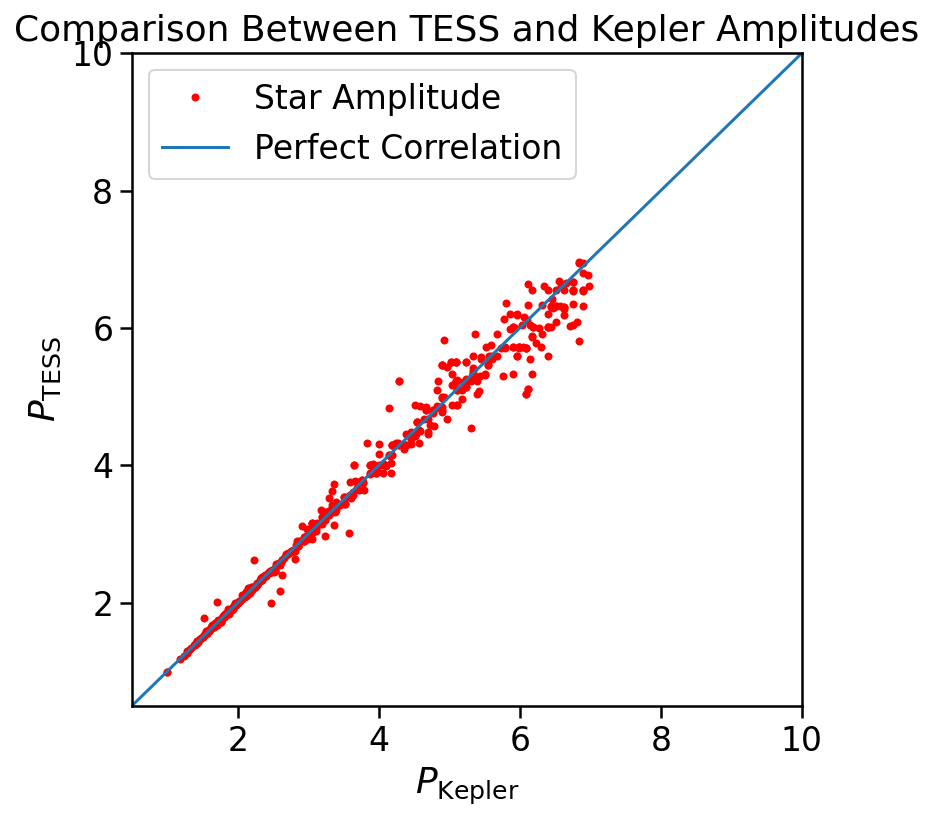
\includegraphics[width=\textwidth]{Comparison Between TESS and Kepler Amplitudes.png}
  \end{figure}

\section{Results}

\subsection{Amplitude versus rotation period for bins in $T_{\mathrm{eff}}$}
  % Helpful resource on how to insert and align images
  % https://www.overleaf.com/learn/latex/Inserting_Images
  \begin{figure}[h]
    \centering
    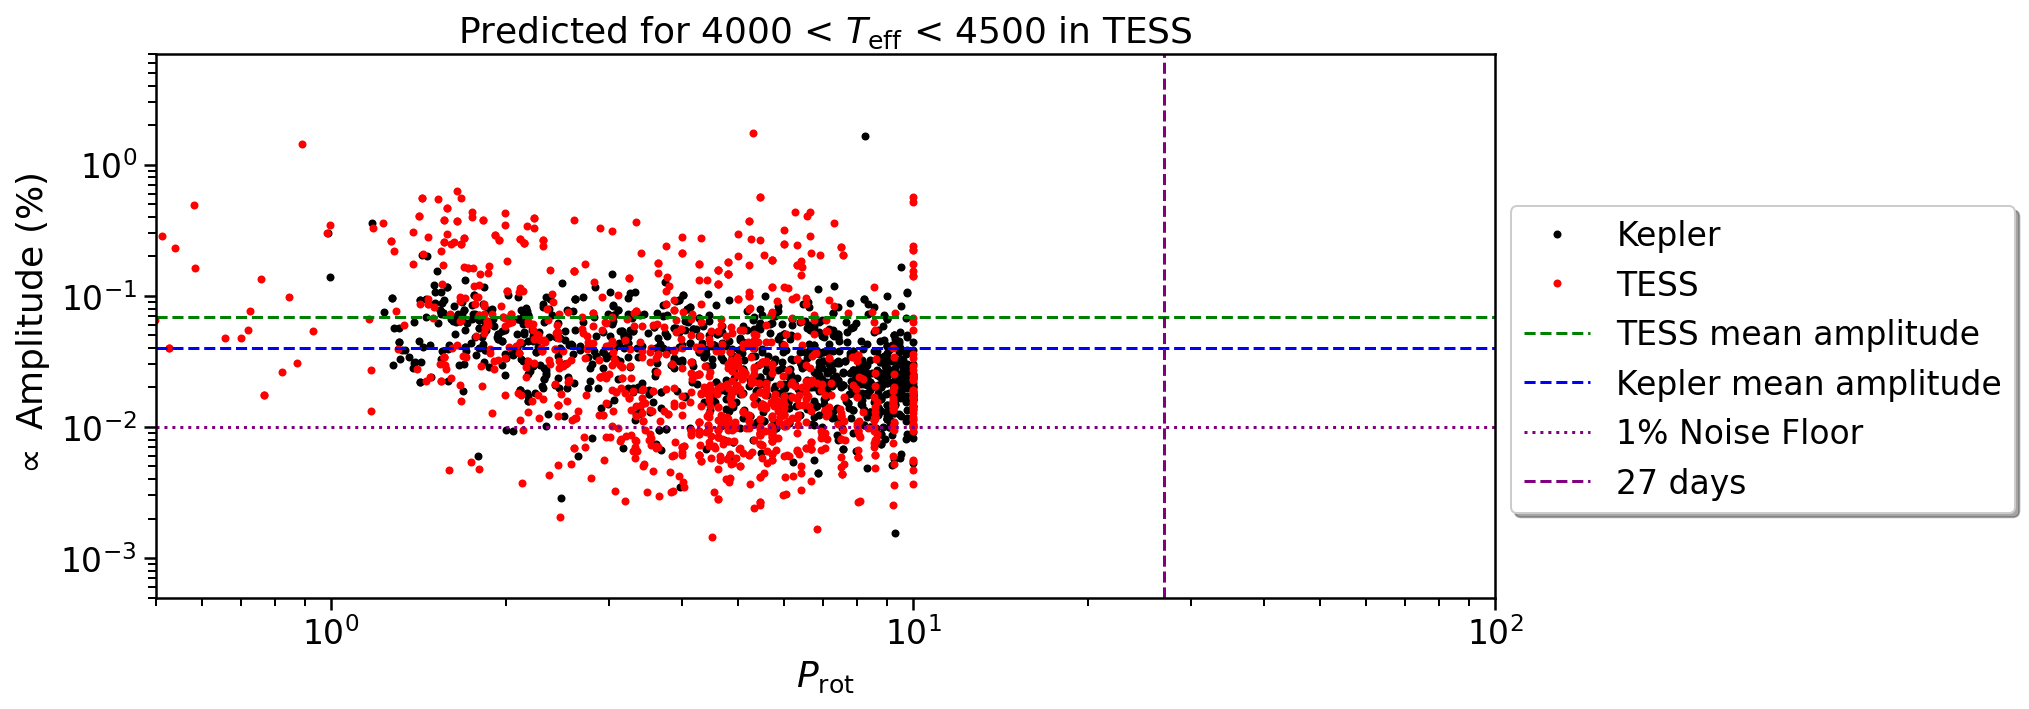
\includegraphics[width=\textwidth]{Amplitude vs. Rotation for Kepler and TESS.png}
  \end{figure}

\subsection{TESS-to-K2 amplitude ratio as a function of $T_{\mathrm{eff}}$}

\subsection{Converting amplitude ratio to $T_{\mathrm{spot}}$}

\subsection{Inferred $T_{\mathrm{spot}}$ versus $T_{\mathrm{eff}}$}



\section{Discussion}

\subsection{Comparison to other studies}
\citet{2016MNRAS.463.2494F} targeted 304 Pleiades sources with LAMOST and found the $T_{\mathrm{spot}}$ scales with $T_{\mathrm{eff}}$ with figure.

\subsection{Assessing the spots versus faculae}
Up to the this point, we have assumed that all flux variations arise from dark spots on the surface of the star. Stars can just as likely have bright patches that cause flux perturbations to their light curves. Here we assess the consequences of assuming faculae instead of spots.

\section{Conclusions}

\begin{acknowledgements}
  This paper includes data collected by the TESS mission. Funding for the TESS mission is provided by the NASA's Science Mission Directorate.

  The authors acknowledge the Texas Advanced Computing Center (TACC, \url{http://www.tacc.utexas.edu}) at The University of Texas at Austin for providing HPC resources that have contributed to the research results reported within this paper.
\end{acknowledgements}

\clearpage


\facilities{Gemini:South, TESS, ASAS, Gaia}

\software{  pandas \citep{mckinney10, reback2020pandas},
  emcee \citep{foreman13},
  matplotlib \citep{hunter07},
  astroplan \citep{astroplan2018},
  astropy \citep{exoplanet:astropy13,exoplanet:astropy18},
  exoplanet \citep{exoplanet:exoplanet},
  numpy \citep{harris2020array},
  scipy \citep{jones01},
  ipython \citep{perez07},
  bokeh \citep{bokehcite},
  seaborn \citep{waskom14}}
%pytorch \citep{NEURIPS2019_9015}} % No pytorch yet!


\bibliography{ms}


\clearpage

\appendix
\restartappendixnumbering

\section{Optional appendix} \label{appendix:tools}

Place optional content here.
\end{document}
